\documentclass[a4paper,12pt]{article}

\title{Physics 30 \\ Electromagnetic Radiation - Optics}
\author{Jad Chehimi}

% document setup
\renewcommand{\familydefault}{\sfdefault}
\linespread{1.25}
\usepackage[margin=1in]{geometry}
\usepackage{setspace}
\usepackage{enumitem}
\setlist{nosep}
\usepackage{color,soul}
\setcounter{secnumdepth}{0}

% tools
\usepackage[hidelinks]{hyperref}
\usepackage{float}
%% images
\usepackage{graphicx}
\graphicspath{ {./images/} }
%% science
\usepackage{siunitx}
\sisetup{exponent-product=\times, per-mode=fraction}

\begin{document}
\maketitle
\tableofcontents

\pagebreak

\section{Terms}
\begin{itemize}
    \item{\textbf{Monochromatic Light}: Light of one colour}
    \item{\textbf{Medium}: the material the wave is travelling in}
    \item{\textbf{Refraction}: a change in the direction of a light wave due to a change in its speed as it passes from one medium to another}
    \item{\textbf{Refractive Index}: a ratio comparing the speed of light in a vacuum to the measured speed of light in a given material ($n = \frac{c}{v}$)}
\end{itemize}

\section{Electromagnetic Spectrum}
\begin{figure}[H]
    \centering
    \caption{"Cosmic" rays on the left of gamma}
    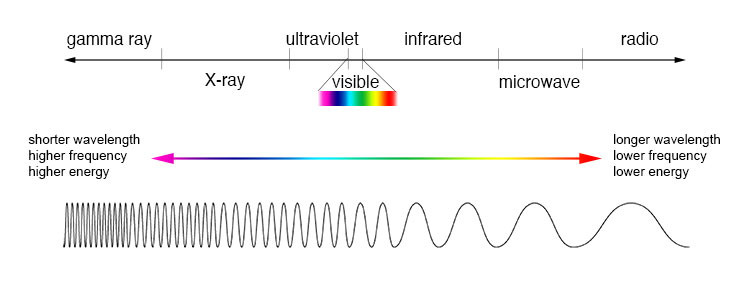
\includegraphics[width=\textwidth]{emr}
\end{figure}
\begin{itemize}
    \item{ALL EMR travels at the speed of light in a vacuum. ($c = \SI{3.00e8}{\m\per\s}$)}
    \item{
        \hl{Memorize the visible spectrum wavelength range}
        \begin{itemize}
            \item{\SI{400}{\nano\m} to \SI{750}{\nano\m}}
            \item{\SI{400e-9}{\m} to \SI{750e-9}{\m}}
        \end{itemize}
    }
\end{itemize}

\subsection{Universal Wave Equation}
\Large $$v = f\lambda$$ \normalsize
\begin{itemize}
    \item{$v$ = speed (\si{\m\per\s})}
    \item{$f$ = frequency (\si{\Hz})}
    \item{$\lambda$ = wavelength (\si{\m}) (often given in nanometers, $\SI{100}{\nano\m} = \SI{100e-9}{\m}$)}
\end{itemize}

Speed of light: $c = f\lambda$

Period: $T = \frac{1}{f}$

\subsection{Transverse Wave}
\begin{figure}[H]
    \centering
    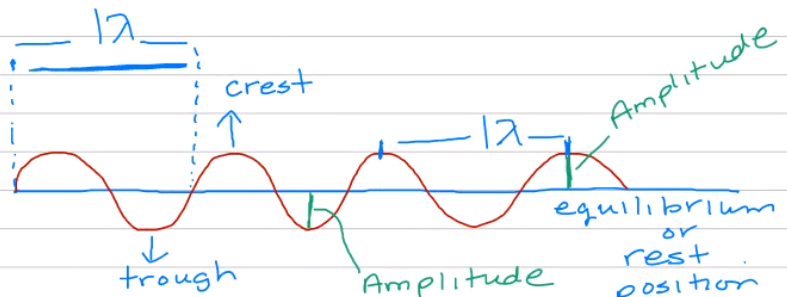
\includegraphics[width=0.9\textwidth]{transverse}
\end{figure}
\begin{itemize}
    \item{\textbf{Crest}: peak of wave}
    \item{\textbf{Trough}: depression of wave}
    \item{\textbf{Amplitude}: the maximum displacement from the equilibrium position}
\end{itemize}

\section{Refraction}
The bending of a wave when entering a new medium at an angle.

\begin{itemize}
    \item{$n$: Index of Refraction (air is $n = \num{1.00}$)}
    \item{When a light ray travels from a lower $n$-value medium to a greater $n$-value medium, the light ray will \hl{bend toward the normal}}
\end{itemize}

\subsection{Snell's Law}
\Large $$n_1\sin{\theta_1} = n_2\sin{\theta_2}$$ \normalsize
Use to calculate the new angle in a different medium/n value.

\Large $$\frac{n_2}{n_1} = \frac{\sin{\theta_1}}{\sin{\theta_2}} = \frac{\lambda_1}{\lambda_2} = \frac{v_1}{v_2}$$ \normalsize

\subsection{Frequency}
Frequency is \hl{unaffected by medium}. 

Frequency can only be changed at the source.

\subsection{Critical Angle}
For any two mediums, the critical angle is the angle of the incident angle for which the angle of refraction is \ang{90}.

Two conditions must be met for a critical angle.
\begin{itemize}
    \item{The light must travel from a \hl{greater $n$-value to a lesser $n$-value}}
    \item{The angle of refraction must be \ang{90.0}}
\end{itemize}
\begin{figure}[H]
    \centering
    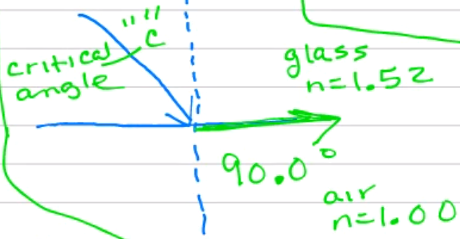
\includegraphics[width=0.50\textwidth]{criticalangle}
\end{figure}

\subsection{Total Internal Reflection}
Reflection of all incident light back into a medium of higher refractive index due to the inability to refract light back at an angle beyond the maximum angle of \ang{90}.

If the angle of incidence is \hl{greater than the critical value}, then the ray will \hl{reflect instead of refract}. (therefore, staying inside the medium)

Trying to calculate this angle with Snell's Law will error.

\subsection{Examples}
\subsubsection{Parallelogram}
\begin{figure}[H]
    \centering
    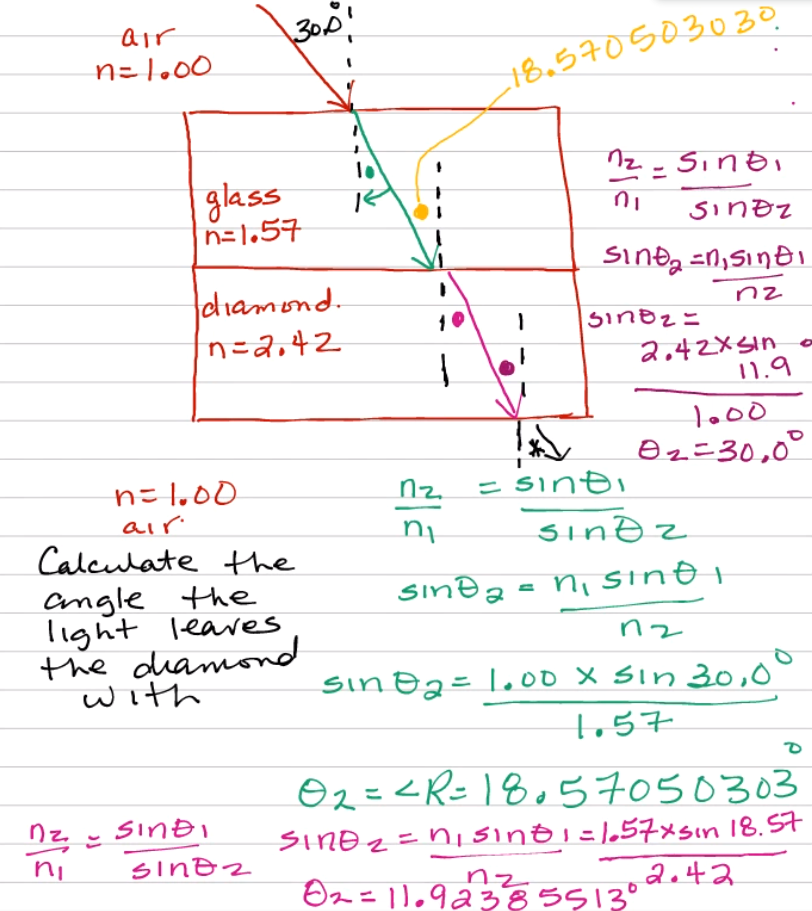
\includegraphics[width=\textwidth]{ex-sqr}
\end{figure}

\subsubsection{Equilateral Triangle}
\begin{figure}[H]
    \centering
    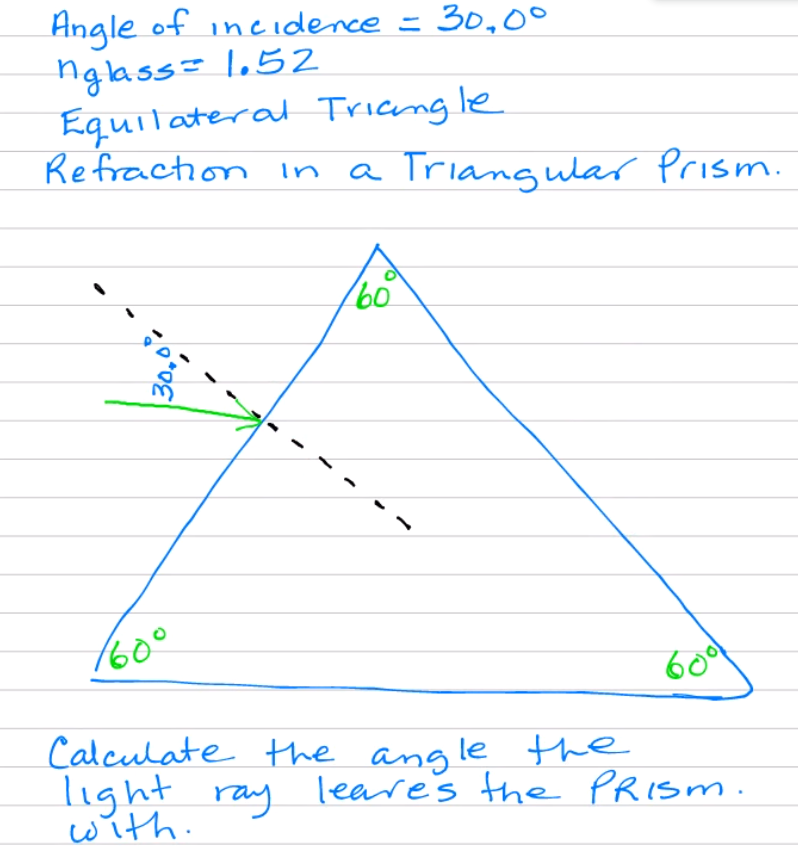
\includegraphics[width=0.45\textwidth]{ex-tri-1}
    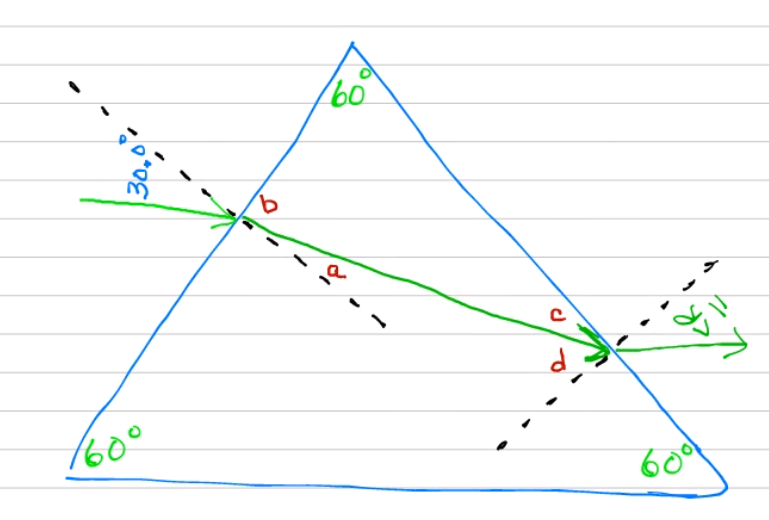
\includegraphics[width=0.45\textwidth]{ex-tri-2}
\end{figure}
\begin{figure}[H]
    \centering
    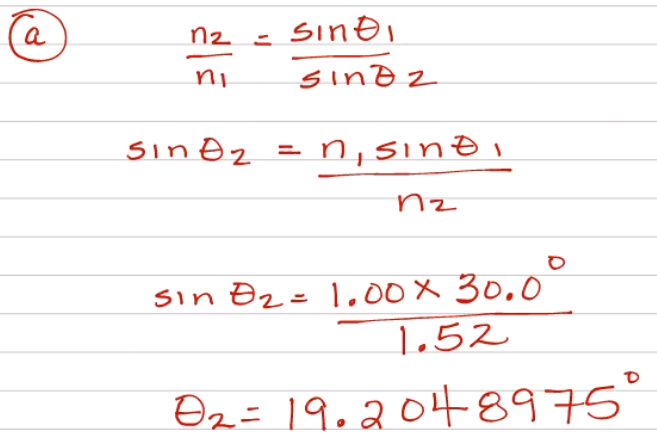
\includegraphics[width=0.45\textwidth]{ex-tri-3}
    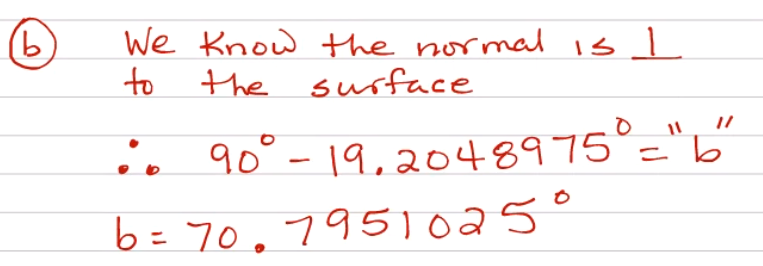
\includegraphics[width=0.45\textwidth]{ex-tri-4}
\end{figure}
\begin{figure}[H]
    \centering
    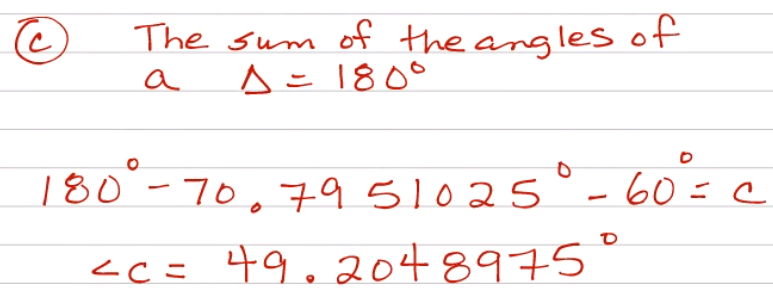
\includegraphics[width=0.45\textwidth]{ex-tri-5}
    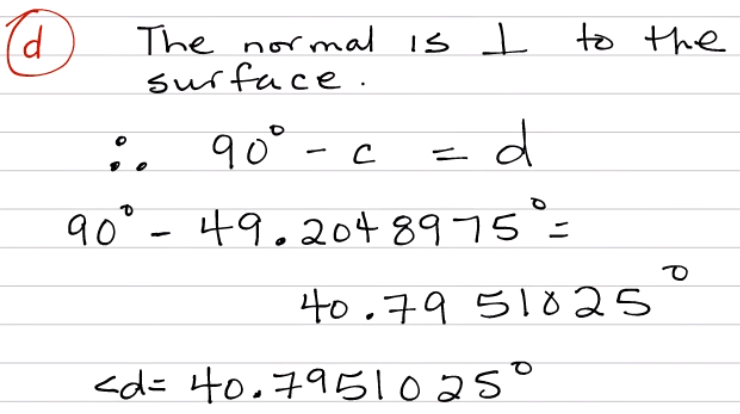
\includegraphics[width=0.45\textwidth]{ex-tri-6}
\end{figure}

$$\theta = \ang{83.3}$$

\pagebreak
\section{Dispersion}
\begin{figure}[H]
    \centering
    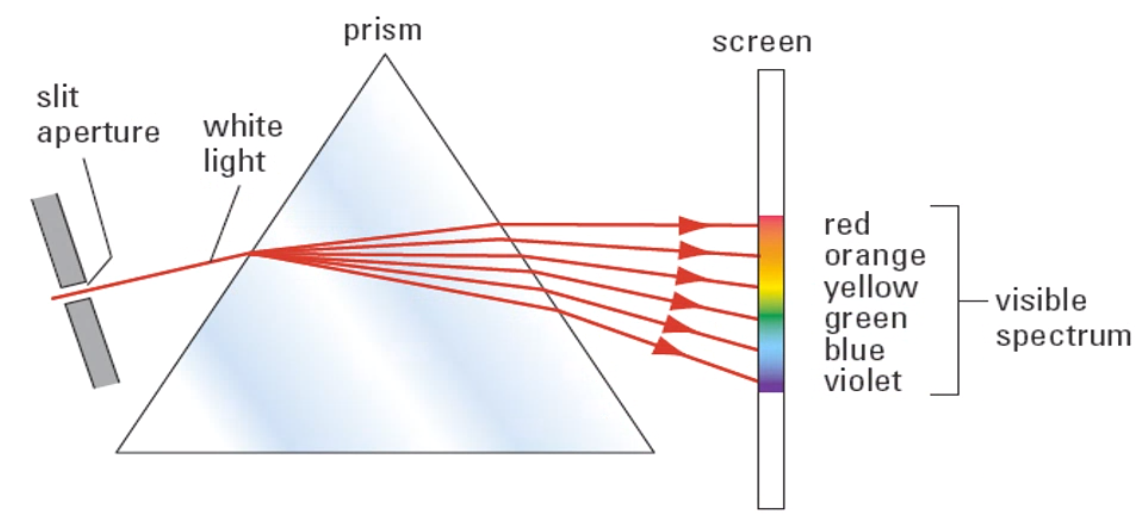
\includegraphics[width=0.8\textwidth]{dispersion}
\end{figure}

Separation of white light into its components.

The refraction of white light to form a spectrum of colours.

\subsection{Spectrum}
The bands of colours making up white light (red, orange, yellow, green, blue, violet)

In a rainbow, light from the sun enters a spherical raindrop and different colors are refracted at different angles.

\subsection{Lens}
A lens is a transmissive optical device that focuses or disperses a light beam by means of refraction.

\pagebreak
\section{Ray Diagrams for Lenses}
\begin{figure}[H]
    \centering
    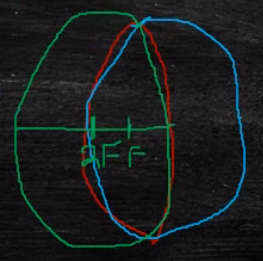
\includegraphics[width=0.50\textwidth]{lens}
    \caption{Red is the lens, comprised of the overlap of two spheres}
\end{figure}
\subsection{Points}
\begin{itemize}
    \item{$F$: The principal focal point, where light rays appear to converge or diverse}
    \item{$C$: Centre of curvature, center of the sphere or the radius, $= 2F$}
\end{itemize}

\subsection{Variables}
\begin{itemize}
    \item{$f$: Focal length (related to the radius of curvature, $f = \frac{\textrm{radius}}{2}$)}
    \item{$m$: Magnification}
    \item{$d_o$: Object distance}
    \item{$d_i$: Image distance}
    \item{$h_o$: Object height}
    \item{$h_i$: Image height}
\end{itemize}

$$\frac{1}{f} = \frac{1}{d_o} + \frac{1}{d_i}$$
$$m = \frac{h_i}{h_o} = \frac{-d_i}{d_o}$$

$f$ is positive for convex lenses.
$f$ is negative for concave lenses.

\subsection{Rays (Striking Lenses)}
\subsubsection{Ray 1}
\begin{itemize}
    \item{Starts from top of object}
    \item{Travels parallel to principal axis}
    \item{After striking midline of lens, bends towards F}
\end{itemize}

\subsubsection{Ray 2}
\begin{itemize}
    \item{Starts from top of object}
    \item{Travels towards F}
    \item{After striking midline of lens, travels parallel to principal axis}
\end{itemize}

\subsubsection{Ray 3}
\begin{itemize}
    \item{Starts from top of object}
    \item{Travels through optical center of lens}
    \item{Does not refract/bend}
    \item{
        Can be used in any scenario, but only useful if...
        \begin{itemize}
            \item{Convex lens with object at F}
            \item{Concave lens}
        \end{itemize}
    }
\end{itemize}

\pagebreak
\section{Convex (Converging Lens)}

\subsection{Object Beyond C}
\begin{figure}[H]
    \centering
    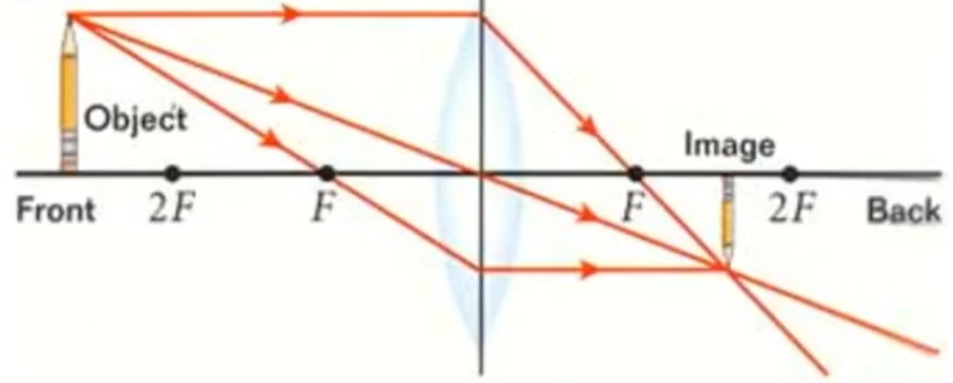
\includegraphics[width=0.8\textwidth]{convex-beyondC}
\end{figure}

\hl{The resulting image can be described as...}
\begin{itemize}
    \item{\textbf{inverted} (upside down)}
    \item{\textbf{diminished} (smaller)}
    \item{located between F and C}
    \item{\textbf{real} (if the object and image are on opposite sides of the lens)}
\end{itemize}

\subsubsection{Example}
A \SI{3.00}{\cm} tall object is placed \SI{30.0}{\cm} in front of a convex lens with a focal length of \SI{10.0}{\cm}. Calculate $d_i$, $h_i$ and $m$.
\begin{figure}[H]
    \centering
    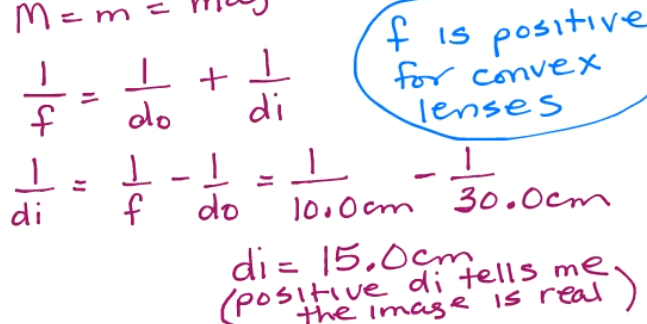
\includegraphics[width=0.45\textwidth]{ex-convex-1}
    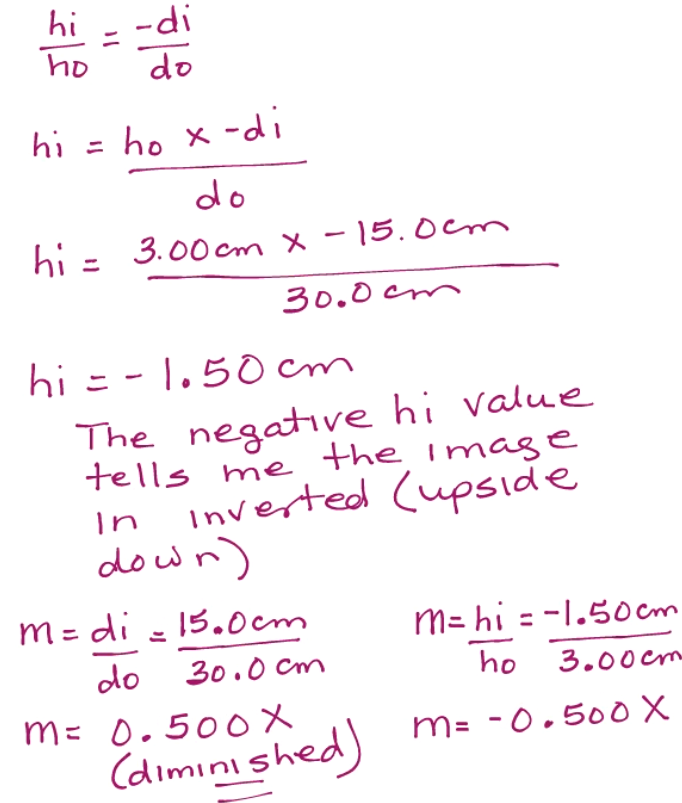
\includegraphics[width=0.45\textwidth]{ex-convex-2}
\end{figure}

\pagebreak
\subsection{Object At C}
\begin{figure}[H]
    \centering
    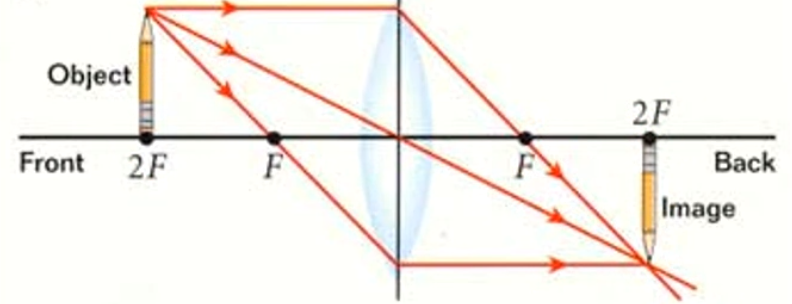
\includegraphics[width=0.75\textwidth]{convex-atC}
\end{figure}

\hl{The resulting image can be described as...}
\begin{itemize}
    \item{inverted}
    \item{same size}
    \item{located at C/2F}
    \item{real}
\end{itemize}

\subsubsection{Example}
A \SI{2.00}{\cm} tall object is placed \SI{20.0}{\cm} in front of a convex lens with a focal length of \SI{10.0}{\cm}. Calculate $d_i$, $h_i$ and $m$.
\begin{itemize}
    \item{$h_o = \SI{2.00}{\cm}$}
    \item{$d_o = \SI{20.0}{\cm}$}
    \item{$f = \SI{10.0}{\cm}$}
\end{itemize}
$$\frac{1}{f} = \frac{1}{d_o} + \frac{1}{d_i}$$
$$\frac{1}{d_i} = \frac{1}{f} - \frac{1}{d_o}$$
$$\frac{1}{d_i} = \frac{1}{\SI{10.0}{\cm}} - \frac{1}{\SI{20.0}{\cm}} = \SI{20.0}{\cm}$$

$$\frac{h_i}{h_o} = \frac{-d_i}{d_o}$$
$$h_i = \frac{h_o \times -d_i}{d_o}$$
$$h_i = \frac{\SI{2.00}{\cm} \times \SI{-20.0}{\cm}}{\SI{20.0}{\cm}} = \SI{2.00}{\cm}$$

$$m = \frac{d_i}{d_o}$$
$$m = \frac{\SI{20.0}{\cm}}{\SI{20.0}{\cm}} = 1$$

\pagebreak
\subsection{Object Between C and F}
\begin{figure}[H]
    \centering
    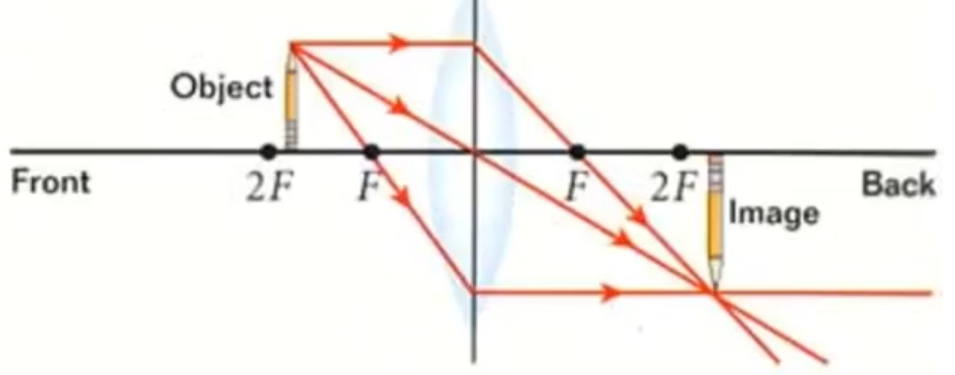
\includegraphics[width=0.8\textwidth]{convex-betweenCandF}
\end{figure}

\hl{The resulting image can be described as...}
\begin{itemize}
    \item{inverted}
    \item{enlarged}
    \item{located beyond C/2F}
    \item{real}
\end{itemize}

\pagebreak
\subsection{Object At F}
\begin{figure}[H]
    \centering
    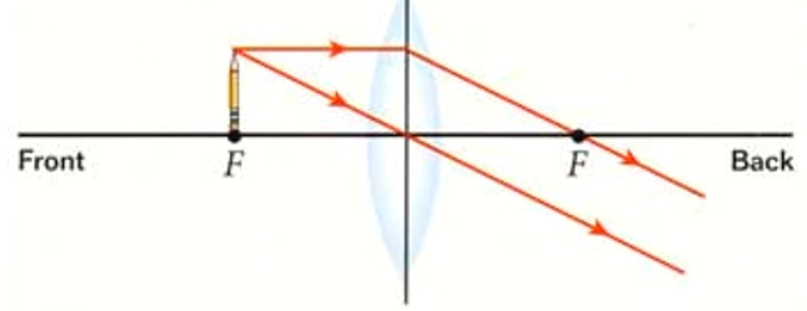
\includegraphics[width=0.7\textwidth]{convex-atF}
    \caption{\hl{Ray 2 cannot be used} because the object is sitting on the focal point (F). We must use Ray 3.}
\end{figure}

The rays end up running parallel to each other, so there is \hl{no image}/\hl{image at infinity}.

\subsection{Object Within F}
\begin{figure}[H]
    \centering
    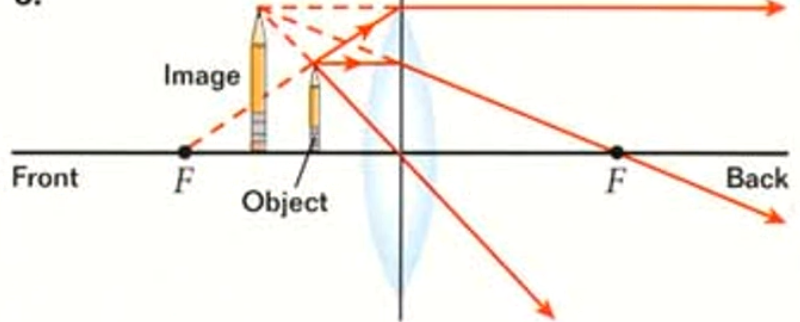
\includegraphics[width=0.7\textwidth]{convex-withinF}
    \caption{The rays on their own don't form a coherent image. Continue the \textbf{refracted} rays \hl{backwards} (dotted lines) so they converge.}
\end{figure}

\hl{The resulting image can be described as...}
\begin{itemize}
    \item{\textbf{erect} (right side up)}
    \item{enlarged}
    \item{located beyond C/2F}
    \item{\textbf{virtual} (object and image on same side)}
\end{itemize}

\pagebreak
\subsubsection{Example}
A \SI{4.00}{\cm} tall object is \SI{20.0}{\cm} in front of a convex lens with a focal length of \SI{40.0}{\cm}. Calculate $d_i$, $h_i$ and $m$.
\begin{itemize}
    \item{$h_o = \SI{4.00}{\cm}$}
    \item{$d_o = \SI{20.0}{\cm}$}
    \item{$f = \SI{40.0}{\cm}$}
\end{itemize}
$$\frac{1}{f} = \frac{1}{d_o} = \frac{1}{d_i}$$
$$\frac{1}{d_i} = \frac{1}{f} - \frac{1}{d_o}$$
$$\frac{1}{d_i} = \frac{1}{\SI{40.0}{\cm}} - \frac{1}{\SI{20.0}{\cm}}$$
$$d_i = \SI{-40.0}{\cm}$$
Negative $d_i$ tells me the image is virtual.

$$\frac{h_i}{h_o} = \frac{-d_i}{d_o}$$
$$h_i = \frac{h_o \times -d_i}{d_o}$$
$$h_i = \frac{\SI{4.00}{\cm} \times -(\SI{-40.0}{\cm})}{\SI{20.0}{\cm}}$$
$$h_i = \SI{8.00}{\cm}$$
Positive $h_i$ means image is erect.

$$m = \frac{h_i}{h_o}$$
$$m = \frac{\SI{8.00}{\cm}}{\SI{4.00}{\cm}}$$
$$m = \num{2.00}$$
Image will be 2.00X bigger than object.

\pagebreak
\section{Concave (Diverging Lens)}
\begin{figure}[H]
    \centering
    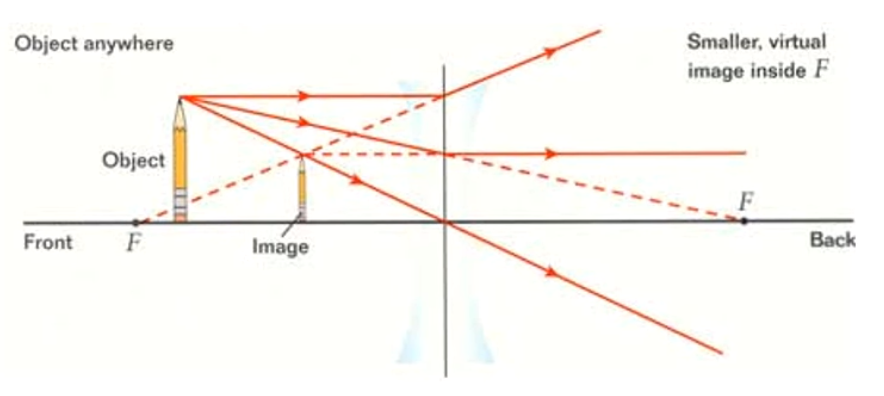
\includegraphics[width=0.75\textwidth]{concave}
\end{figure}

\hl{Concave lenses ALWAYS result in images described as...}
\begin{itemize}
    \item{erect}
    \item{diminished}
    \item{virtual}
\end{itemize}

\subsection{Example}
A \SI{4.00}{\cm} tall object is \SI{15.0}{\cm} in front of a concave lens with a focal length of \SI{12.0}{\cm}. Calculate $d_i$, $h_i$, and $m$.
\begin{itemize}
    \item{$h_o = \SI{4.00}{\cm}$}
    \item{$d_o = \SI{15.0}{\cm}$}
    \item{$f = \SI{-12.0}{\cm}$}
\end{itemize}

$$\frac{1}{f} = \frac{1}{d_o} = \frac{1}{d_i}$$
$$\frac{1}{d_i} = \frac{1}{f} - \frac{1}{d_o}$$
$$\frac{1}{d_i} = \frac{1}{\SI{-12.0}{\cm}} - \frac{1}{\SI{15.0}{\cm}}$$
$d_i = \SI{-6.67}{\cm}$ (virtual)

$$\frac{h_i}{h_o} = \frac{-d_i}{d_o}$$
$$h_i = \frac{h_o \times -d_i}{d_o}$$
$$h_i = \frac{\SI{4.00}{\cm} \times -(\SI{-6.67}{\cm})}{\SI{15.0}{\cm}}$$
$h_i = \SI{1.78}{\cm}$ (erect)

$$m = \frac{h_i}{h_o}$$
$$m = \frac{\SI{1.78}{\cm}}{\SI{4.00}{\cm}}$$
$m = \num{0.444}$ (diminished)

\pagebreak
\section{Reflection}
\subsection{Law of Reflection}

\Large $$\theta_I = \theta_R$$ \normalsize

\begin{figure}[H]
    \centering
    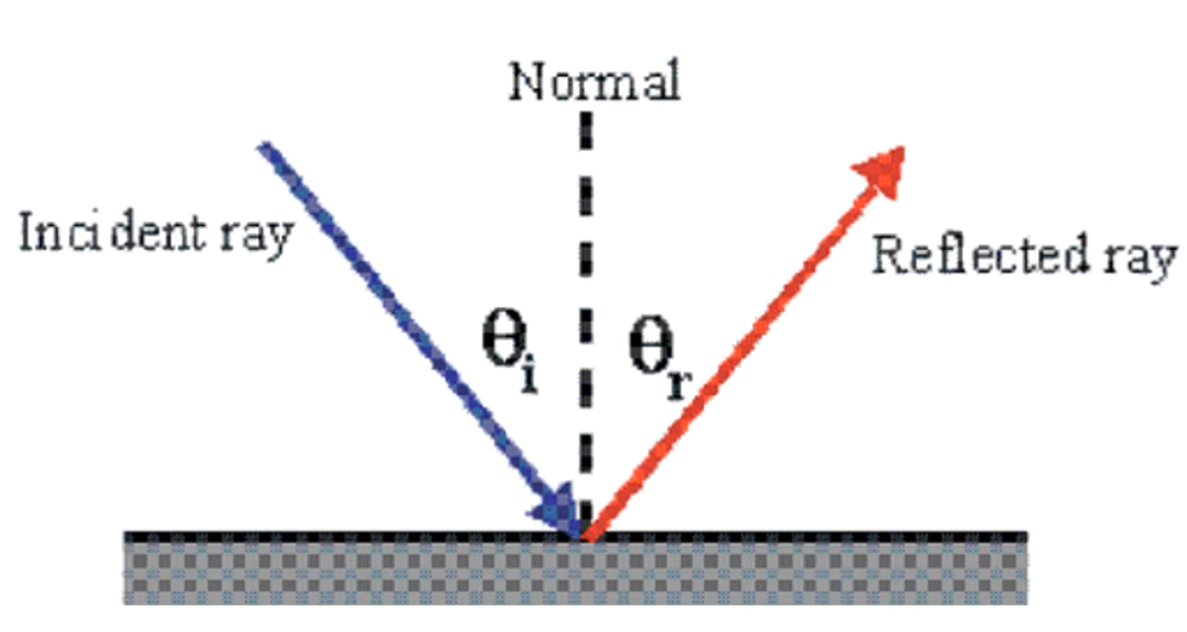
\includegraphics[width=0.45\textwidth]{reflectangles}
    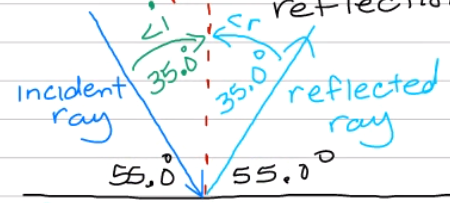
\includegraphics[width=0.45\textwidth]{reflect}
\end{figure}

\begin{itemize}
    \item{$\theta_I$: \textbf{Angle of Incidence} \\Measured from the light ray to the normal}
    \item{$\theta_R$: \textbf{Angle of Reflection} \\Measured from reflected ray to normal}
\end{itemize}

\subsubsection{Normal}
\begin{itemize}
    \item{Perpendicular to the surface}
    \item{Broken/dotted line}
    \item{Drawn from where the incident ray contacts the mirror surface}
    \item{All angles are always measured with respect to the normal}
\end{itemize}

\subsubsection{Example}
A light ray strikes a flat mirror at an angle of \ang{70.0} to the mirror surface. What is the angle of reflection? What is the angle between the incident ray and the reflected ray?
\begin{figure}[H]
    \centering
    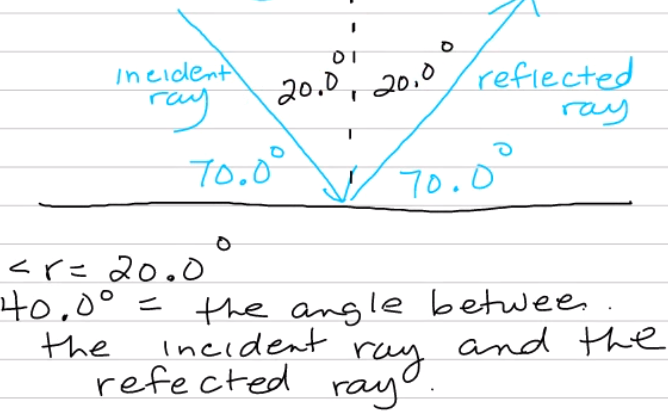
\includegraphics[width=0.6\textwidth]{ex-reflect}
\end{figure}

\subsection{Type of Reflections}
\begin{figure}[H]
    \centering
    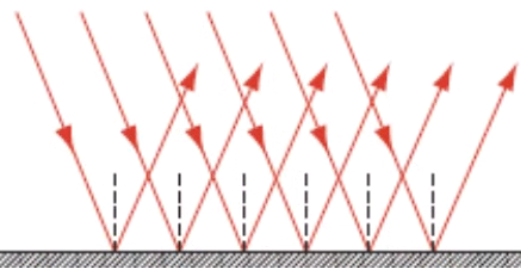
\includegraphics[width=0.45\textwidth]{specular-reflection}
    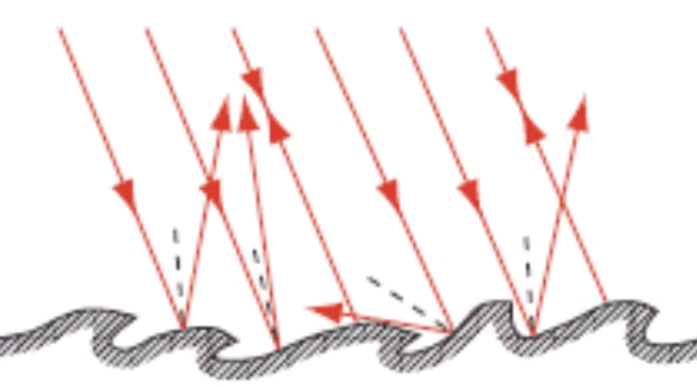
\includegraphics[width=0.45\textwidth]{diffuse-reflection}
    \caption{Left = specular (regular) reflection, Right = diffuse (irregular) reflection}
\end{figure}

\subsection{Plane Mirror}
A smooth, flat (planar) reflecting surface

$\theta_R = \theta_I$, angle of reflection equals angle of incidence

\subsubsection{Properties}
\begin{itemize}
    \item{\hl{Erect} (right side up)}
    \item{\hl{Same size}}
    \item{\hl{Equal distance} from mirror to object and mirror to image}
    \item{\hl{Laterally reversed} (from right to left)}
    \item{\hl{Virtual image} (inside the mirror)}
\end{itemize}

\textbf{Virtual Image}: An image from which light rays appear to come; cannot be formed on a non-reflective surface or screen.

\pagebreak

\section{Mirrors}

\subsection{Rays (Striking Mirrors)}
\subsubsection{Ray 1}
\begin{itemize}
    \item{Starts from top of object}
    \item{Travels parallel to principal axis}
    \item{After striking mirror, reflects back towards F}
\end{itemize}

\subsubsection{Ray 2}
\begin{itemize}
    \item{Starts from top of object}
    \item{Travels towards F}
    \item{After striking mirror, reflects back parallel to principal axis}
\end{itemize}

\subsubsection{Ray 3}
\begin{itemize}
    \item{Starts from C, travels up towards top of object}
    \item{From top of object to mirror, maintain angle}
    \item{Does not refract/bend}
    \item{
        Can be used in any scenario, but only useful if...
        \begin{itemize}
            \item{Concave mirror with object at F}
        \end{itemize}
    }
\end{itemize}

\section{Concave Mirrors}
\begin{itemize}
    \item{$f$ is positive for concave mirrors}
    \item{Concave mirrors are \hl{converging mirrors}}
\end{itemize}

\subsection{Object Beyond C}
\begin{figure}[H]
    \centering
    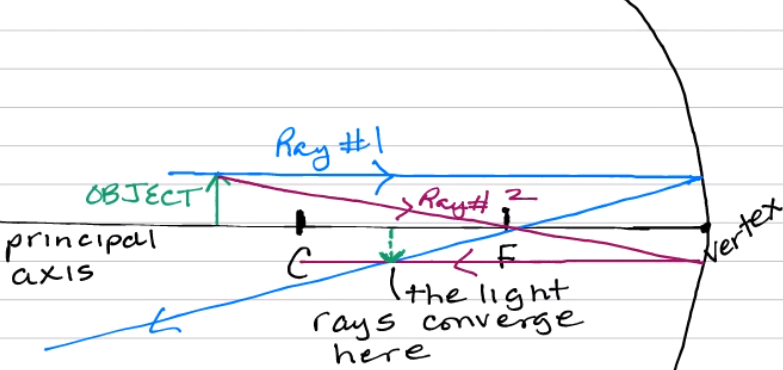
\includegraphics[width=0.8\textwidth]{concave-mirror-beyondC}
\end{figure}
\hl{The resulting image can be described as...}
\begin{itemize}
    \item{\textbf{inverted} (upside down)}
    \item{\textbf{diminished} (smaller)}
    \item{located between C and F}
    \item{\textbf{real} (\hl{in front of mirror})}
\end{itemize}

\subsection{Object At C}
\begin{figure}[H]
    \centering
    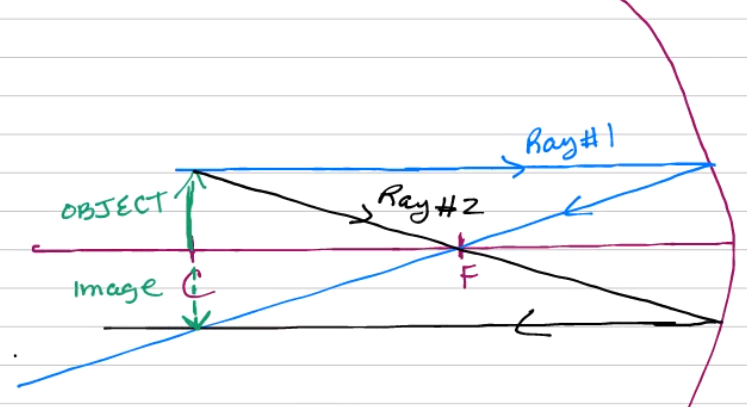
\includegraphics[width=0.8\textwidth]{concave-mirror-atC}
\end{figure}
\hl{The resulting image can be described as...}
\begin{itemize}
    \item{\textbf{inverted}}
    \item{\textbf{same size}}
    \item{located at C}
    \item{\textbf{real}}
\end{itemize}

\subsection{Object Between C and F}
\begin{figure}[H]
    \centering
    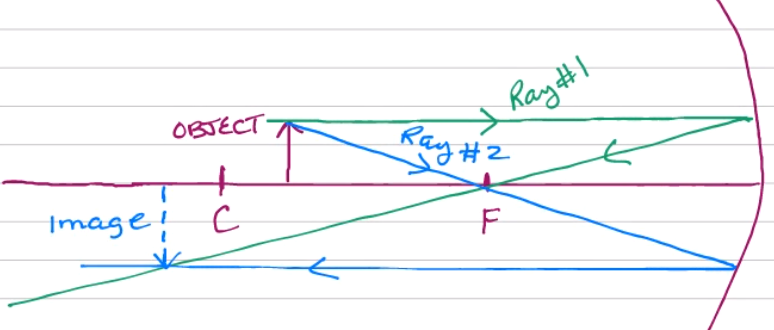
\includegraphics[width=0.8\textwidth]{concave-mirror-betweenCandF}
\end{figure}
\hl{The resulting image can be described as...}
\begin{itemize}
    \item{\textbf{inverted}}
    \item{\textbf{enlarged}}
    \item{located beyond C}
    \item{\textbf{real}}
\end{itemize}

\subsubsection{Example}
An object \SI{3.00}{\cm} tall is located \SI{15.0}{\cm} from a concave mirror with a focal length of \SI{10.0}{\cm}. Calculate $d_i$, $h_i$, and $m$.
\begin{itemize}
    \item{$h_o = \SI{3.00}{\cm}$}
    \item{$d_o = \SI{15.0}{\cm}$}
    \item{$f = \SI{10.0}{\cm}$}
\end{itemize}
$$\frac{1}{f} = \frac{1}{d_o} + \frac{1}{d_i}$$
$$\frac{1}{d_i} = \frac{1}{f} - \frac{1}{d_o}$$
$$\frac{1}{d_i} = \frac{1}{\SI{10.0}{\cm}} - \frac{1}{\SI{15.0}{\cm}}$$
$d_i = \SI{30.0}{\cm}$ (positive $d_i$ = image is real)

$$\frac{h_i}{h_o} = \frac{-d_i}{d_o}$$
$$h_i = \frac{h_o \times -d_i}{d_o}$$
$$h_i = \frac{\SI{3.00}{\cm} \times \SI{-30.0}{\cm}}{\SI{15.0}{\cm}}$$
$h_i = \SI{-6.00}{\cm}$ (negative $h_i$ = image is inverted)

$$m = \frac{d_i}{d_o}$$
$$m = \frac{\SI{30.0}{\cm}}{\SI{15.0}{\cm}}$$
$m = \num{2.00}$ (image is enlarged 2.00X)

\subsection{Object At F}
\begin{figure}[H]
    \centering
    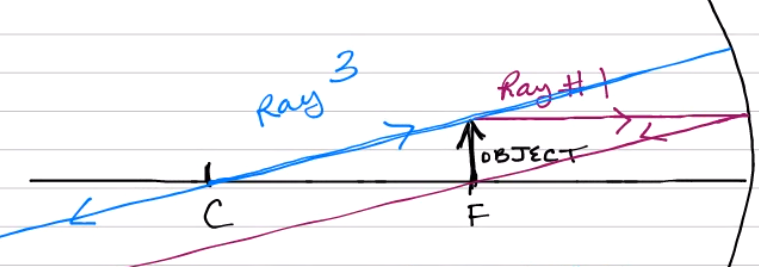
\includegraphics[width=0.8\textwidth]{concave-mirror-atF}
\end{figure}

The rays end up running parallel to each other, so there is \hl{no image}/\hl{image at infinity}.

\subsection{Object Within F}
\begin{figure}[H]
    \centering
    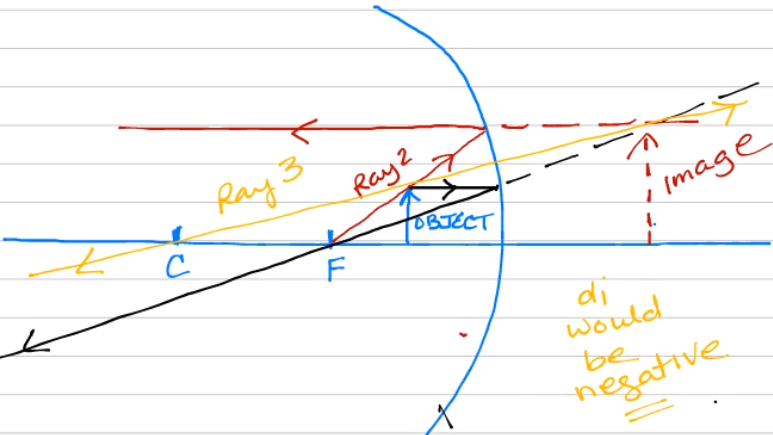
\includegraphics[width=0.8\textwidth]{concave-mirror-withinF}
\end{figure}
\hl{The resulting image can be described as...}
\begin{itemize}
    \item{\textbf{erect}}
    \item{\textbf{enlarged}}
    \item{\textbf{virtual}}
\end{itemize}

\subsubsection{Example}
A \SI{2.00}{\cm} tall object is placed \SI{5.00}{\cm} in front of a concave mirror with a focal length of \SI{10.0}{\cm}. Calculate $d_i$, $h_i$, and $m$.
\begin{itemize}
    \item{$h_o = \SI{2.00}{\cm}$}
    \item{$d_o = \SI{5.00}{\cm}$}
    \item{$f = \SI{10.0}{\cm}$}
\end{itemize}
$$\frac{1}{f} = \frac{1}{d_o} + \frac{1}{d_i}$$
$$\frac{1}{d_i} = \frac{1}{f} - \frac{1}{d_o}$$
$$\frac{1}{d_i} = \frac{1}{\SI{10.0}{\cm}} - \frac{1}{\SI{5.00}{\cm}}$$
$d_i = \SI{-10.0}{\cm}$ (negative $d_i$ = image is virtual)

$$\frac{h_i}{h_o} = \frac{-d_i}{d_o}$$
$$h_i = \frac{h_o \times -d_i}{d_o}$$
$$h_i = \frac{\SI{2.00}{\cm} \times -(\SI{-10.0}{\cm})}{\SI{5.00}{\cm}}$$
$h_i = \SI{4.00}{\cm}$ (positive $h_i$ = image is erect)

$$m = \frac{d_i}{d_o}$$
$$m = \frac{\SI{4.00}{\cm}}{\SI{2.00}{\cm}}$$
$m = \num{2.00}$ (image is enlarged 2.00X)

\pagebreak
\section{Convex Mirror}
\begin{itemize}
    \item{$f$ is negative for convex mirrors}
    \item{Convex mirrors are \hl{diverging mirrors}}
\end{itemize}

\begin{figure}[H]
    \centering
    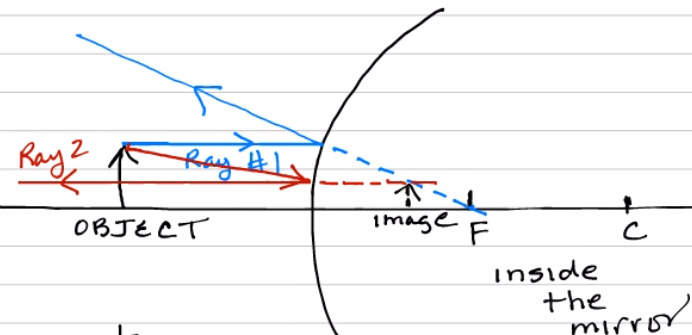
\includegraphics[width=0.8\textwidth]{convex-mirror}
\end{figure}
\hl{The resulting image can be described as...}
\begin{itemize}
    \item{\textbf{erect}}
    \item{\textbf{diminished}}
    \item{\textbf{virtual}}
\end{itemize}

\subsection{Example}
A \SI{4.00}{\cm} tall object is placed \SI{12.0}{\cm} in front of a convex mirror with a focal length of \SI{15.0}{\cm}. Calculate $d_i$, $h_i$, and $m$.
\begin{itemize}
    \item{$h_o = \SI{4.00}{\cm}$}
    \item{$d_o = \SI{12.0}{\cm}$}
    \item{$f = \SI{-15.0}{\cm}$}
\end{itemize}
$$\frac{1}{f} = \frac{1}{d_o} + \frac{1}{d_i}$$
$$\frac{1}{d_i} = \frac{1}{f} - \frac{1}{d_o}$$
$$\frac{1}{d_i} = \frac{1}{\SI{-15.0}{\cm}} - \frac{1}{\SI{12.0}{\cm}}$$
$d_i = \SI{-6.67}{\cm}$ (negative $d_i$ = image is virtual)

$$\frac{h_i}{h_o} = \frac{-d_i}{d_o}$$
$$h_i = \frac{h_o \times -d_i}{d_o}$$
$$h_i = \frac{\SI{4.00}{\cm} \times -(\SI{-6.67}{\cm})}{\SI{12.0}{\cm}}$$
$h_i = \SI{2.22}{\cm}$ (positive $h_i$ = image is erect)

$$m = \frac{d_i}{d_o}$$
$$m = \frac{\SI{2.22}{\cm}}{\SI{4.00}{\cm}}$$
$m = \num{0.56}$ (image is diminished 0.56X)

\section{Diffraction}
The slight bending of light as it passes around the edge of an object.

Change in shape and direction of a wave front as a result of encountering a small opening or aperture in a barrier.
\begin{figure}[H]
    \centering
    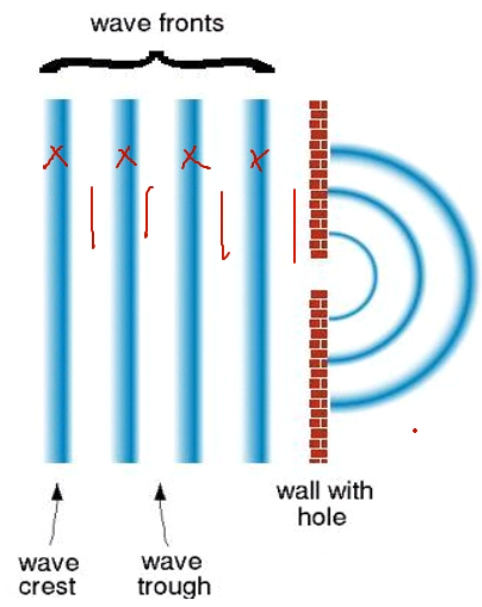
\includegraphics[width=0.50\textwidth]{diffraction}
\end{figure}

\section{Interference (Superposition)}
\begin{figure}[H]
    \centering
    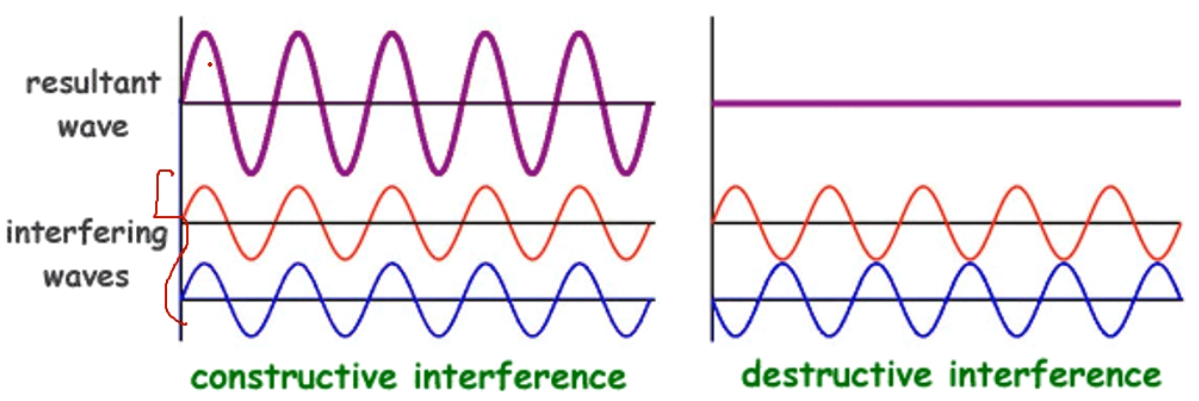
\includegraphics[width=\textwidth]{interference}
\end{figure}
\subsection{Constructive}
When crest meets crest or trough meets trough.

Produces a pulse of \hl{greater amplitude}. (sum)
\begin{figure}[H]
    \centering
    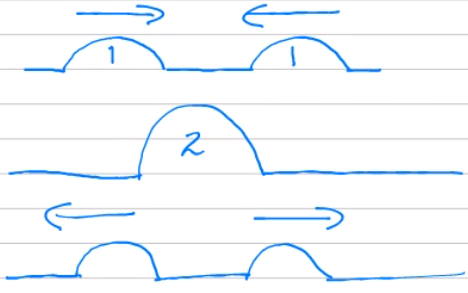
\includegraphics[width=0.50\textwidth]{constructive-interference}
\end{figure}

\subsection{Destructive}
When crest meets trough.

Produces a pulse of \hl{lesser amplitude}. (sum)
\begin{figure}[H]
    \centering
    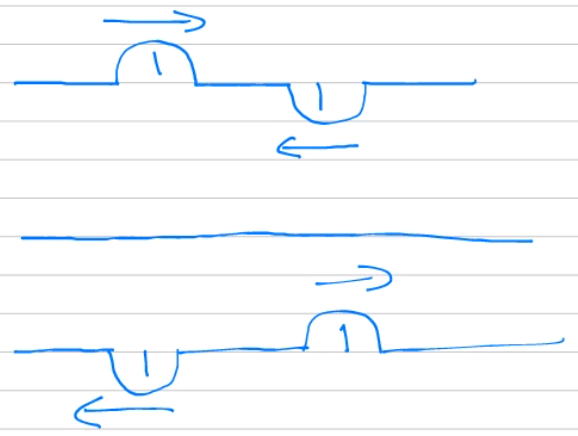
\includegraphics[width=0.50\textwidth]{destructive-interference}
\end{figure}

\subsection{Diffraction-Interferance}
\begin{figure}[H]
    \centering
    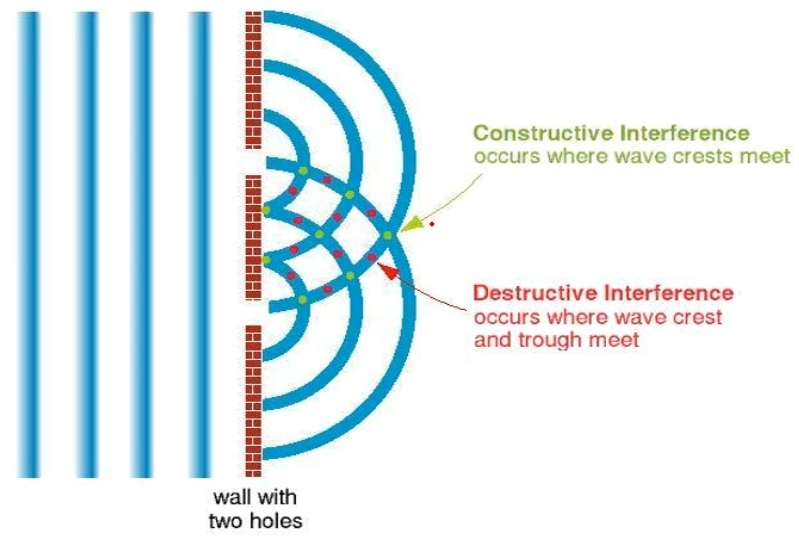
\includegraphics[width=\textwidth]{interdiff}
\end{figure}

\subsection{Standing Wave}
\begin{figure}[H]
    \centering
    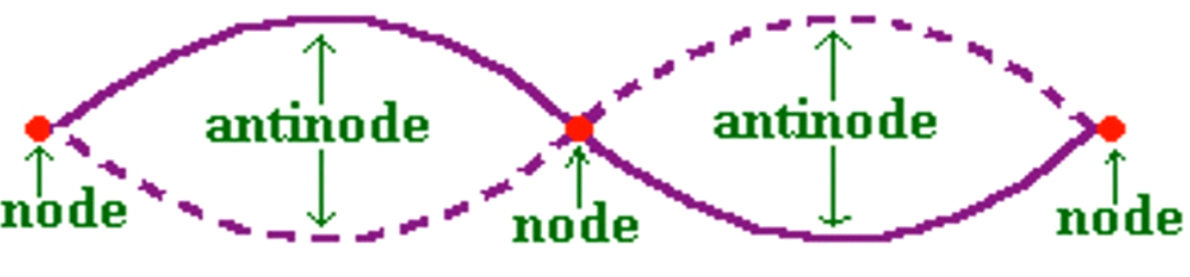
\includegraphics[width=0.75\textwidth]{standing-wave}
    \caption{Solid: Incident pulse, Dotted: Reflected pulse}
\end{figure}
A standing wave, also known as a stationary wave, is a wave which oscillates in time but whose peak amplitude profile does not move in space.

\begin{itemize}
    \item{\textbf{Antinode}: \\The point of interaction between waves in which \hl{only constructive interference} occurs}
    \item{\textbf{Node}: \\The point of interaction between waves in which \hl{only destructive interference} occurs}
\end{itemize}

Each node type is half a wavelength between eachother.

\section{Thomas Young Diffraction-Interferance Experiment}
Thomas Young's experiment \hl{supports only the light is a wave theory}. (test question) Light travels in straight lines, but it is a wave that can be diffracted and interferred.

If light was a particle, you'd expect the light to go straight through two slits and form two spots on a screen. This does not occur.
\begin{figure}[H]
    \centering
    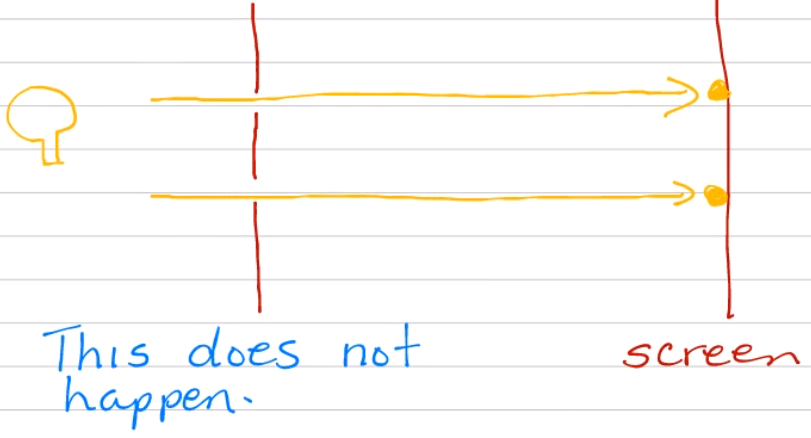
\includegraphics[width=0.4\textwidth]{experiment-1}
\end{figure}

What actually occurs is the light waves diffract and form bands.
\begin{figure}[H]
    \centering
    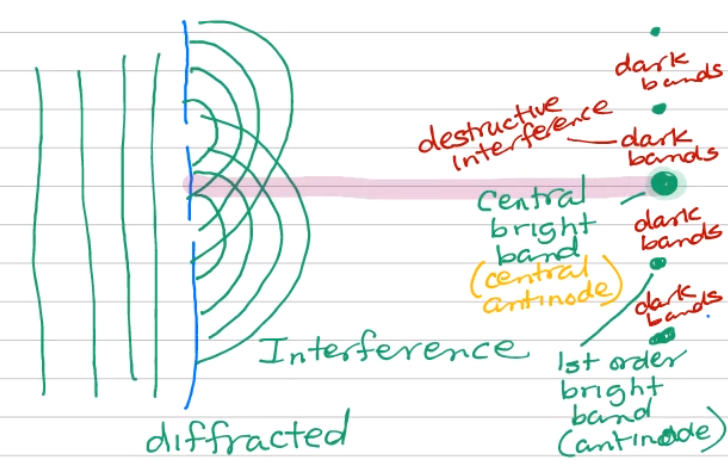
\includegraphics[width=0.6\textwidth]{experiment-2}
    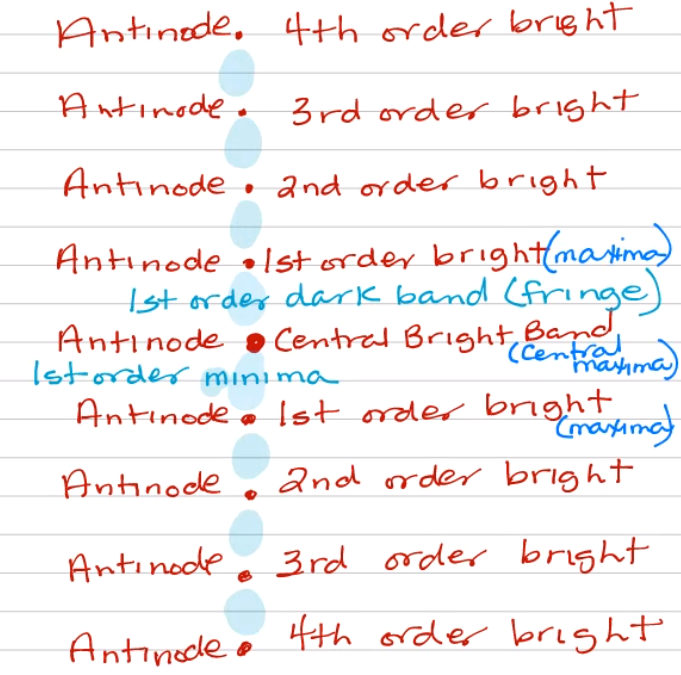
\includegraphics[width=0.35\textwidth]{experiment-3}
\end{figure}
\begin{itemize}
    \item{\textbf{Bright Bands}: Regions of constructive interference (green dots) (aka. antinode, maxima)}
    \item{\textbf{Dark Bands}: Regions of destructive interference (space between green dots) (aka. node, minima)}
\end{itemize}

\begin{figure}[H]
    \centering
    \caption{The position of the two waves varies depending on path length, and this determines if their intersection is an antinode or node}
    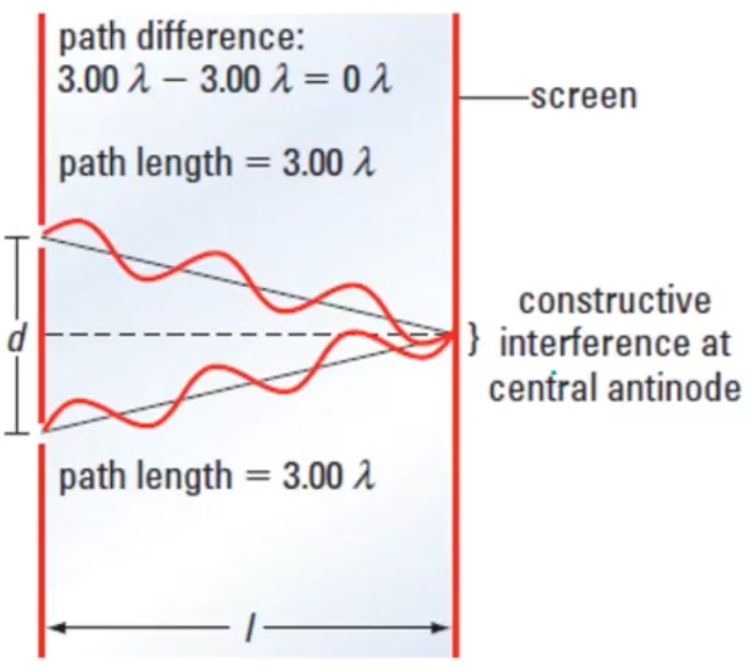
\includegraphics[width=0.325\textwidth]{slit1}
    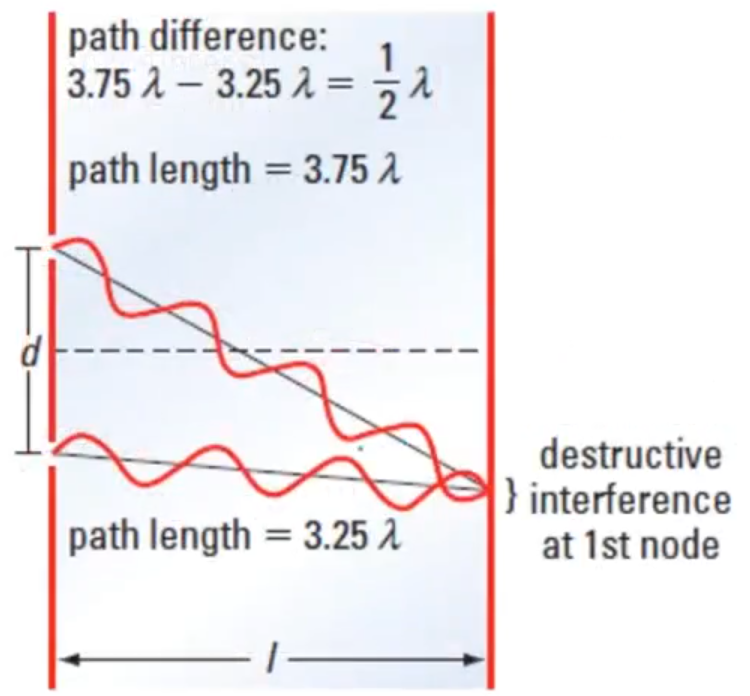
\includegraphics[width=0.325\textwidth]{slit2}
    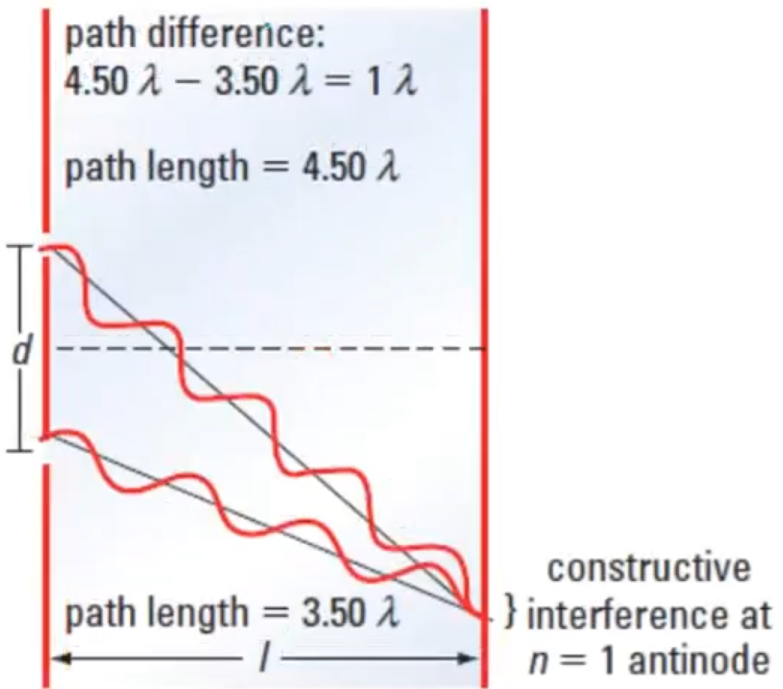
\includegraphics[width=0.325\textwidth]{slit3}
    \caption{1st: Waves of light after 2 slits forming central antinode, notice both waves are same (form a trough) at the antinode, constructive}
    \caption{2nd: Waves of light after 2 slits forming 1st node, notice both waves are different (crest/trough), destructive}
    \caption{3rd: Waves of light after 2 slits forming 1st antinode, notice both waves are same (form a crest) at the antinode, constructive}
\end{figure}

$n$ is the difference of path lengths, and is used to determine nodes and antinodes.
\begin{itemize}
    \item{Bright to bright: $n$ increases by \num{1}}
    \item{Dark to dark: $n$ increases by \num{1}}
    \item{Bright to dark: $n$ increases by \num{0.5}}
\end{itemize}

\pagebreak
\subsection{Equations}
\begin{figure}[H]
    \centering
    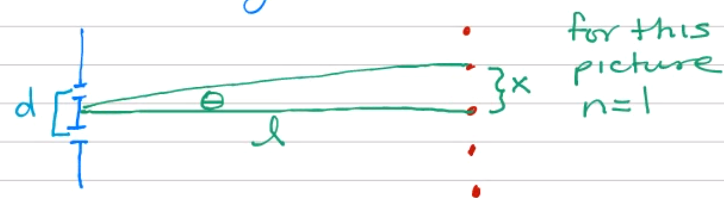
\includegraphics[width=\textwidth]{lighteq}
\end{figure}

\Large $$\lambda = \frac{d\sin{\theta}}{n}$$ \normalsize
\begin{itemize}
    \item{$\lambda$ = wavelength (\si{\m})}
    \item{$d$ = distance between the slits (\si{\m})}
    \item{$\theta$ = angle in degrees}
    \item{$n$ = number of images (bright/dark bands) included in calculation}
\end{itemize}

\Large $$\lambda = \frac{xd}{nl}$$ \normalsize 
($\theta$ must be \hl{less than} \ang{10} to use this equation, angle can be checked with $\tan{\theta} = \frac{x}{l}$)
\begin{itemize}
    \item{$\lambda$ = wavelength (\si{\m})}
    \item{$x$ = distance between images (bright/dark bands) included in calculation}
    \item{$d$ = distance between the slits (\si{\m})}
    \item{$n$ = number of images (bright/dark bands) included}
    \item{$l$ = length to the screen (\si{\m})}
\end{itemize}

\subsection{Tips}
\begin{itemize}
    \item{If you are given lines per meter, \hl{the reciprocal is $d$}}
    \item{In order to get the \hl{maximum number of maxima}, solve for $n$ when the angle is \ang{90.0}}
\end{itemize}

\pagebreak
\subsection{Example}
A screen is \SI{1.20}{\m} from two narrow slits. The slits are a distance of \SI{3.00e-5}{\m} apart. The second order maxima is \SI{4.50e-2}{\m} from the central maximum. Determine the wavelength of light.
\begin{itemize}
    \item{$l$ = \SI{1.20}{\m}}
    \item{$d = \SI{3.00e-5}{\m}$}
    \item{$x = \SI{4.00e-2}{\m}$}
    \item{$n = 2$}
\end{itemize}

$$\tan{\theta} = \frac{ \SI{4.50e-2}{\m} }{ \SI{1.20}{\m} }$$
$\theta = \ang{2.15}$ (less than \ang{10}, either equation may be used)

$$\lambda = \frac{xd}{nl} = \frac{ (\SI{4.50e-2}{\m})(\SI{3.00e-5}{\m}) }{ (\num{2})(\SI{1.20}{\m}) } = \SI{5.63e-7}{\m}$$

\subsection{Example II}
Monochromatic light falls on 2 slits \SI{0.0200}{\milli\m} apart producing a 4th order maximum at \ang{6.40} angle. What is the wavelength of light?
\begin{itemize}
    \item{$d = \SI{0.0200e-3}{\m}$}
    \item{$\theta = \ang{6.40}$}
    \item{$n = 4$}
\end{itemize}

$$\lambda = \frac{d\sin{\theta}}{n} = \frac{ (\SI{0.0200e-3}{\m})(\sin{\ang{6.40}}) }{ \num{4} } = \SI{5.57e-7}{\m}$$

\subsection{Example III}
A diffraction grating has \num{550} lines per \si{\milli\m}. A first order maximum is produced \SI{0.131}{\m} from the central bright band when the screen is \SI{0.342}{\m} from the grating. Determine the wavelength of light.
\begin{itemize}
    \item{$x = \SI{0.131}{\m}$}
    \item{$d = \frac{1}{\SI{550000}{lines\per\m}}{\si{\m}} = \SI{1.818e-6}{\m}$}
    \item{$n = 1$}
    \item{$l = \SI{0.342}{\m}$}
\end{itemize}

$$\tan{\theta} = \frac{ \SI{0.131}{\m} }{ \SI{0.342}{\m} }$$
$\theta = \ang{20.96}$ (greater than \ang{10}, only first equation may be used)

$$\lambda = \frac{d\sin{\theta}}{n} = \frac{ (\SI{1.818e-6}{\m})(\sin{\ang{20.96}}) }{ \num{1} } = \SI{6.50e-7}{\m}$$

\subsection{Example IV}
A diffraction grating has \SI{5.00e5}{lines\per\m}. How many maxima can be observed if the grating is illuminated with monochromatic light of wavelength \SI{4.50e-7}{\m}.
\begin{itemize}
    \item{$\theta = \ang{90.0}$ (in order to get the \hl{maximum number of maxima}, the angle must be \ang{90.0})}
    \item{$\lambda = \SI{4.50e-7}{\m}$}
    \item{$d = \frac{1}{\SI{5.00e5}{lines\per\m}}$}
\end{itemize}
$$n = \frac{ d \sin{\theta} }{ \lambda } = \frac{ (\frac{1}{\SI{5.00e5}{lines\per\m}})(\sin{\ang{90.0}}) }{ \SI{4.50e-7}{\m} } = 4$$

\section{Michelson's Experiment}
Michelson attempted to find the speed of light using the following apparatus.
\begin{figure}[H]
    \centering
    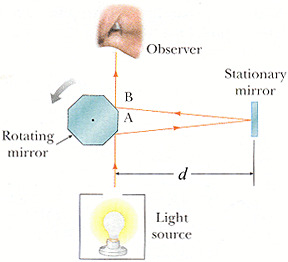
\includegraphics[width=0.50\textwidth]{michelson}
\end{figure}
The light reflects off a typically spinning 8-sided mirror twice (B to mirror to A) so any \hl{distance} used in calculations must be \hl{multiplied by two}.

\subsection{Example}
If an eight-sided mirror makes \SI{420}{RPS}, how long does it take to make one-eighth of a revolution?
$$\frac{\SI{420}{R}}{\SI{1}{\s}} = \frac{\SI{1/8}{R}}{x \si{\s}}$$
$$x = \SI{2.98e-4}{\s}$$

\subsection{Example II}
An eight-sided mirror displayed an image when rotating at \SI{3.12e4}{RPM}, what is the speed of light if the fixed mirror was placed \SI{35.0}{\km} from the rotating mirror?
$$v = \frac{d}{t}$$

$d = \SI{35000}{\m} \times 2$ (light travels from rotating to stationary and back, so x2)

$$\frac{ \SI{3.12e4}{R} }{ \SI{60}{\s} } = \frac{\SI{1/8}{R}}{x \si{\s}}$$
$$x = \SI{2.40e-4}{\s}$$

$$v = \frac{\SI{70000}{\m}}{\SI{2.40e-4}{\s}} = \SI{2.91e8}{\m\per\s}$$

\subsection{Example III}
An eight-sided mirror and a fixed mirror are \SI{30.0}{\km} apart. What is the minimum angular velocity in revolutions per second that the eight-sided mirror would have to rotate in order that light would be reflected to the observer?

$$v = \frac{d}{t}$$
$$t = \frac{d}{v} = \frac{ \SI{30000}{\m}\times2 }{ \SI{3.00e8}{\m\per\s} } = \SI{2.00e-4}{\s}$$

$$\frac{\SI{1/8}{R}}{\SI{2.00e-4}{\s}} = \frac{x \si{R}}{\SI{1}{\s}}$$
$$x = \SI{625}{RPS}$$

\end{document}
